\section{Running the Tool}
\label{sec:component_diagrams-running}

CODA is an extension of the Rodin Platform. See the Rodin User Handbook  for a full description of how to run the Rodin Platform and how to create and verify Event-B models.


Event-B models (including those with CODA models) can be imported and exported from the Rodin platform. Right-click anywhere in the Event-B Explorer view and select Import from the pop-up menu.
From the select window (Figure \ref{fig:ImportingaModelProject}), select \textbf{\texttt{General - Existing Projects into Workspace}} and click on \textbf{\texttt{Next}}. (DO NOT select \textbf{\texttt{Archive File}}, even if you are about to import a zip file).
 

\begin{figure}[!htbp]
  \centering
  \ifplastex
  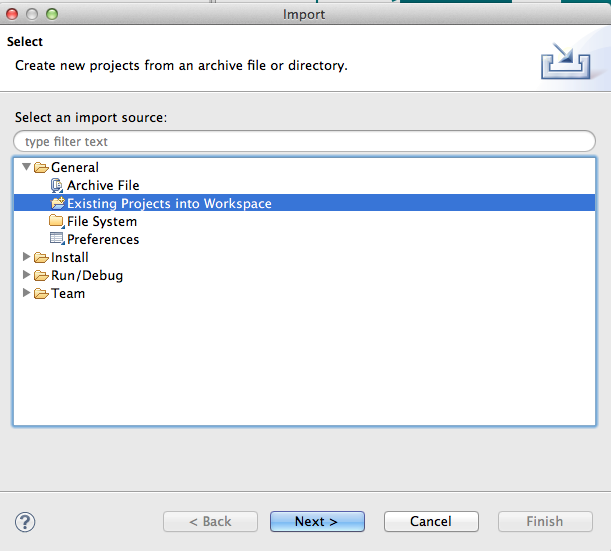
\includegraphics[width=512]{figures/image2.png}
  \else
  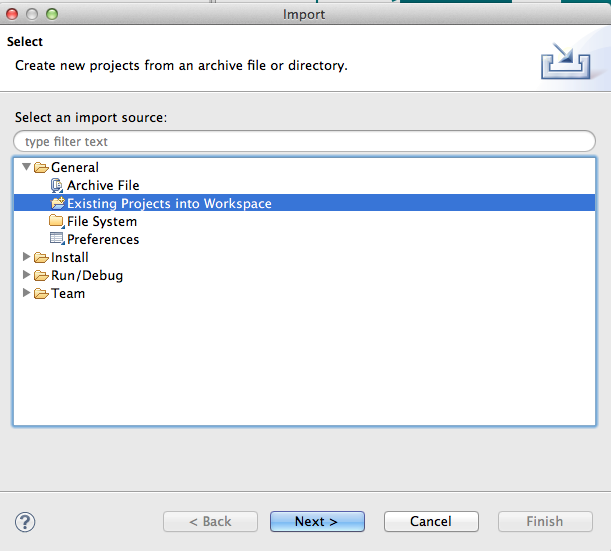
\includegraphics[width=0.5\textwidth]{figures/image2.png}
  \fi
  \caption{Importing a Model Project}
  \label{fig:ImportingaModelProject}
\end{figure}


At the next window, select \textbf{\texttt{Select archive file}} and browse to your archived file. Any projects in the archive will be listed for selection in the centre pane of this window. (Make sure that \textbf{\texttt{copy projects into workspace}} is checked otherwise any changes will be made to the original copy). Click on \textbf{\texttt{Finish}}.


To export models, select the project(s) that you want to archive and choose \textbf{\texttt{Export}} from the pop-up menu. From the window that appears, select \textbf{\texttt{General-Archive File}} and press \textbf{\texttt{Next}}. Type in or browse to a location for the archive file and press \textbf{\texttt{Finish}} (Figure \ref{fig:ExportingaModelProject}).
 
\begin{figure}[!htbp]
  \centering
  \ifplastex
  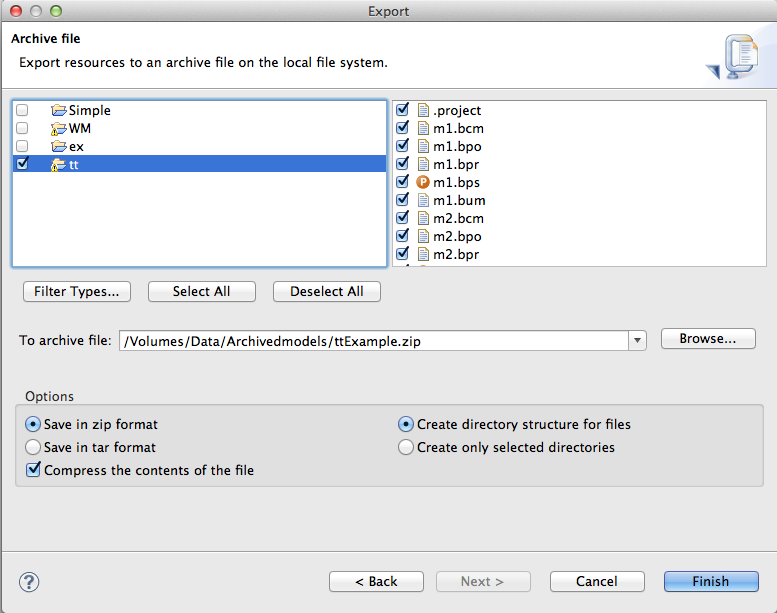
\includegraphics[width=512]{figures/image3.png}
  \else
  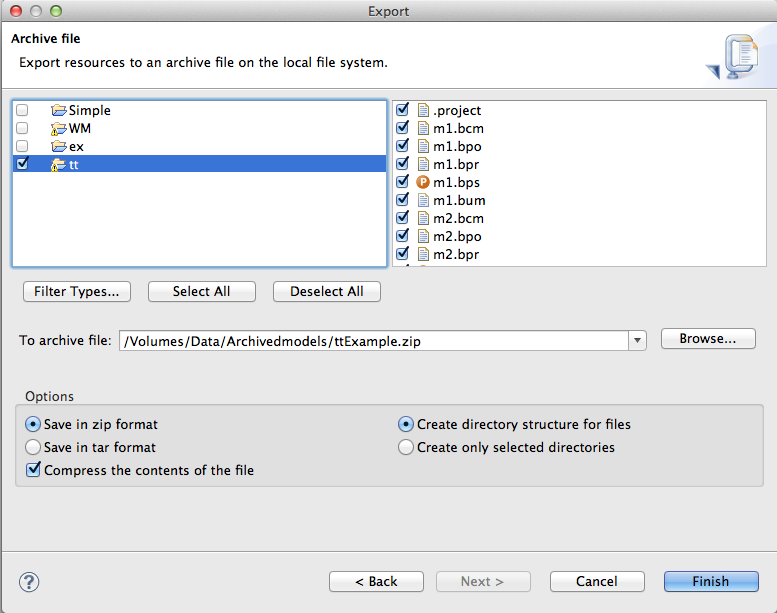
\includegraphics[width=0.5\textwidth]{figures/image3.png}
  \fi
  \caption{Exporting a Model Project}
  \label{fig:ExportingaModelProject}
\end{figure}

%%% Local Variables:
%%% mode: latex
%%% TeX-master: "component_diagrams-user_manual"
%%% End:
